\documentclass[compress]{beamer}
\usepackage[utf8]{inputenc}
\usepackage[english]{babel}
\usepackage{hyperref}
\usepackage{ccicons}

\usepackage{tikz}
\usetikzlibrary{graphs, quotes, arrows.meta, matrix}

\usetheme{default}
\usecolortheme{Nord}
\setbeamertemplate{navigation symbols}{}

\title{Sorting and Searching}
\author{Lorenzo Ferrari, Davide Bartoli}
\date{\today}

\begin{document}

\begin{frame}
  \maketitle
\end{frame}

\begin{frame}{Table of contents}
  \tableofcontents
\end{frame}

\section{Problemi}

\subsection{Subarray Distinct Values}
\begin{frame}{Subarray Distinct Values}
    \begin{exampleblock}{Subarray Distinct Values}
        Dato un array $a$ di $n \leq 2 \cdot 10^5$ interi, conta il numero di subarray con al pi\`u $k$ valori distinti.
    \end{exampleblock}
    \underline{\url{https://cses.fi/problemset/task/2428}}
    \pause
    \begin{itemize}
        \item idee?
        \pause
        \item notiamo che, dato un array con $\leq k$ elementi distinti, anche ogni suo sottoarray ha $\leq k$ elementi distinti
        \pause
        \item per ogni indice $i$, troviamo il massimo $j$ tale che $\{ a_i, a_{i+1}, \dots, a_{j} \}$ ha al pi\`u $k$ elementi distinti.
        \pause
        \item anche tutti i subarray $a[i:i], a[i:i+1], \dots, a[i:j]$ (in totale $j-i+1$) hanno al pi\`u $k$ valori distinti
        \pause
        \item iterando su tutti gli $i$, stiamo contanto tutti i subarray
    \end{itemize}
\end{frame}

\subsection{Tasks and Deadlines}
\begin{frame}{Tasks and Deadlines}
    \underline{\url{https://cses.fi/problemset/task/1630}}
    \pause
    \begin{itemize}
        \item inizialmente il problema sembra complesso, ci sono tante variabili da considerare.
        \pause
        \item un'idea comune in questo tipo di problemi \'e cercare di trovare un ordinamento ottimale (potrebbe non esistere).
        \pause 
\item trovando un ordinamento adatto, potremmo risolvere il problema in $O(n \log n + f(n))$, dove $f(n)$ \`e il costo per processare $n$ elementi ordinati in modo ottimale.
    \end{itemize}
    \vfill
    Idea generalizzata: \url{https://codeforces.com/blog/entry/63533}
\end{frame}

\begin{frame}{Tasks and Deadlines}
    \begin{block}{Dimostrazione}
        Consideriamo il seguente caso: ci troviamo all'istante $k$ e dobbiamo scegliere quale task da fare prima tra $x$ e $y$.
        \begin{itemize}
            \pause
            \item se facciamo prima $x$ allora otteniamo $d_x-(k+a_x)+ d_y-(k+a_x+a_y) = d_x+d_y-2k-2a_x-a_y$
            \item se invece facciamo prima $y$ allora otteniamo $d_y-(k+a_y)+ d_x-(k+a_y+a_x) = d_x+d_y-2k-2a_y-a_x$
            \pause
            \item quando ci conviene fare prima $x$? quando \\ $d_x+d_y-2k-2a_x-a_y \geq d_x+d_y-2k-2a_y-a_x$ \\ \pause $-2a_x-a_y \geq -2a_y-a_x$  \pause \\ $-a_x \geq -a_y$ \\ $a_x \leq a_y$  non dipende da $k$!
        \end{itemize}
    \end{block}
    \pause
    Possiamo ordinare i task in base alla loro durata e risolvere il problema in $O(n \log n)$.
\end{frame}

\subsection{Dangerous Flowers}
\begin{frame}{Problemi}{ois\_antennas}
    \begin{exampleblock}{ois\_antennas}
        $N$ antenne sono in fila. Ognuna \`e caratterizzata dalla sensibilit\`a di $L_i$ decibel, la potenza di $P_i$ decibel e due interi $S_i$, $T_i$.
        \begin{itemize}
            \item l'antenna $i$ riceve un segnale se arriva con una potenza $\geq L_i$ decibel.
            \item ogni antenna pu\`o sempre ricevere segnali, ma trasmette solo negli istanti $S_i, S_i + T_i, S_i + 2T_i,  \dots$
            \item i segnali viaggiano solo verso destra
            \item un segnale raggiunge istantaneamente tutte le antenne, ma la potenza diminuisce di $D$ decibel passando tra due antenne consecutive
        \end{itemize}
        Trova l'istante in cui l'antenna $N-1$ riceve da $0$.
    \end{exampleblock}
    \underline{\url{https://training.olinfo.it/\#/task/ois_antennas/statement}}
\end{frame}

\begin{frame}{Problemi}{ois\_antennas}
    \begin{itemize}
        \item idee?
        \pause
        \item soluzione $O(N^2)$
        \begin{itemize}
            \item processiamo le antenne in ordine
            \item per controllare se e quanto l'antenna $i$ riceve il segnale, controllo quando le antenne $0, 1, \dots, i-1$ trasmettono il segnale
            \item la soluzione \`e corretta, ma non abbastanza efficiente
        \end{itemize}
    \end{itemize}
    \pause
    \textbf{osservazione:} un segnale $(p_a, t_a)$ che arriva al tempo $t_a$ con potenza $p_a$, \`e sicuramente meglio di tutti i segnali $(p_b, t_b)$ con $p_a > p_b$ e $t_a < t_b$.
    \pause
    Al contrario non possiamo dire nulla su due segnali $(p_a, t_a), (p_b, t_b)$ con $p_a > p_b$ e $t_a > t_b$.
\end{frame}


\begin{frame}{Problemi}{ois\_antennas}
    Risolviamo il subtask $D = 0$, quello in cui la potenza non diminuisce viaggiando tra antenne successive.
    \begin{itemize}
        \item teniamo un set dei segnali \textit{potenzialmente} migliori, ossia un set $(p_a, t_b), (p_b, t_b), \dots , (p_k, t_k)$ con $p_a < p_b < \dots < p_k$ e $t_a < t_b < \dots < t_k$.
        \pause
        \item dobbiamo scrivere una struttura dati che supporti:
        \pause
        \begin{itemize}
            \item inserimento di una coppia $(p, t)$
            \begin{itemize}
                \item complessit\`a $O(\log n)$ ammortizzato
            \end{itemize}
            \pause
            \item trovare il primo segnale con potenza $\geq L_i$
            \begin{itemize}
                \item complessit\`a $O(\log n)$
            \end{itemize}
        \end{itemize}
    \end{itemize}
\end{frame}

\begin{frame}{}
    \makebox[\textwidth]{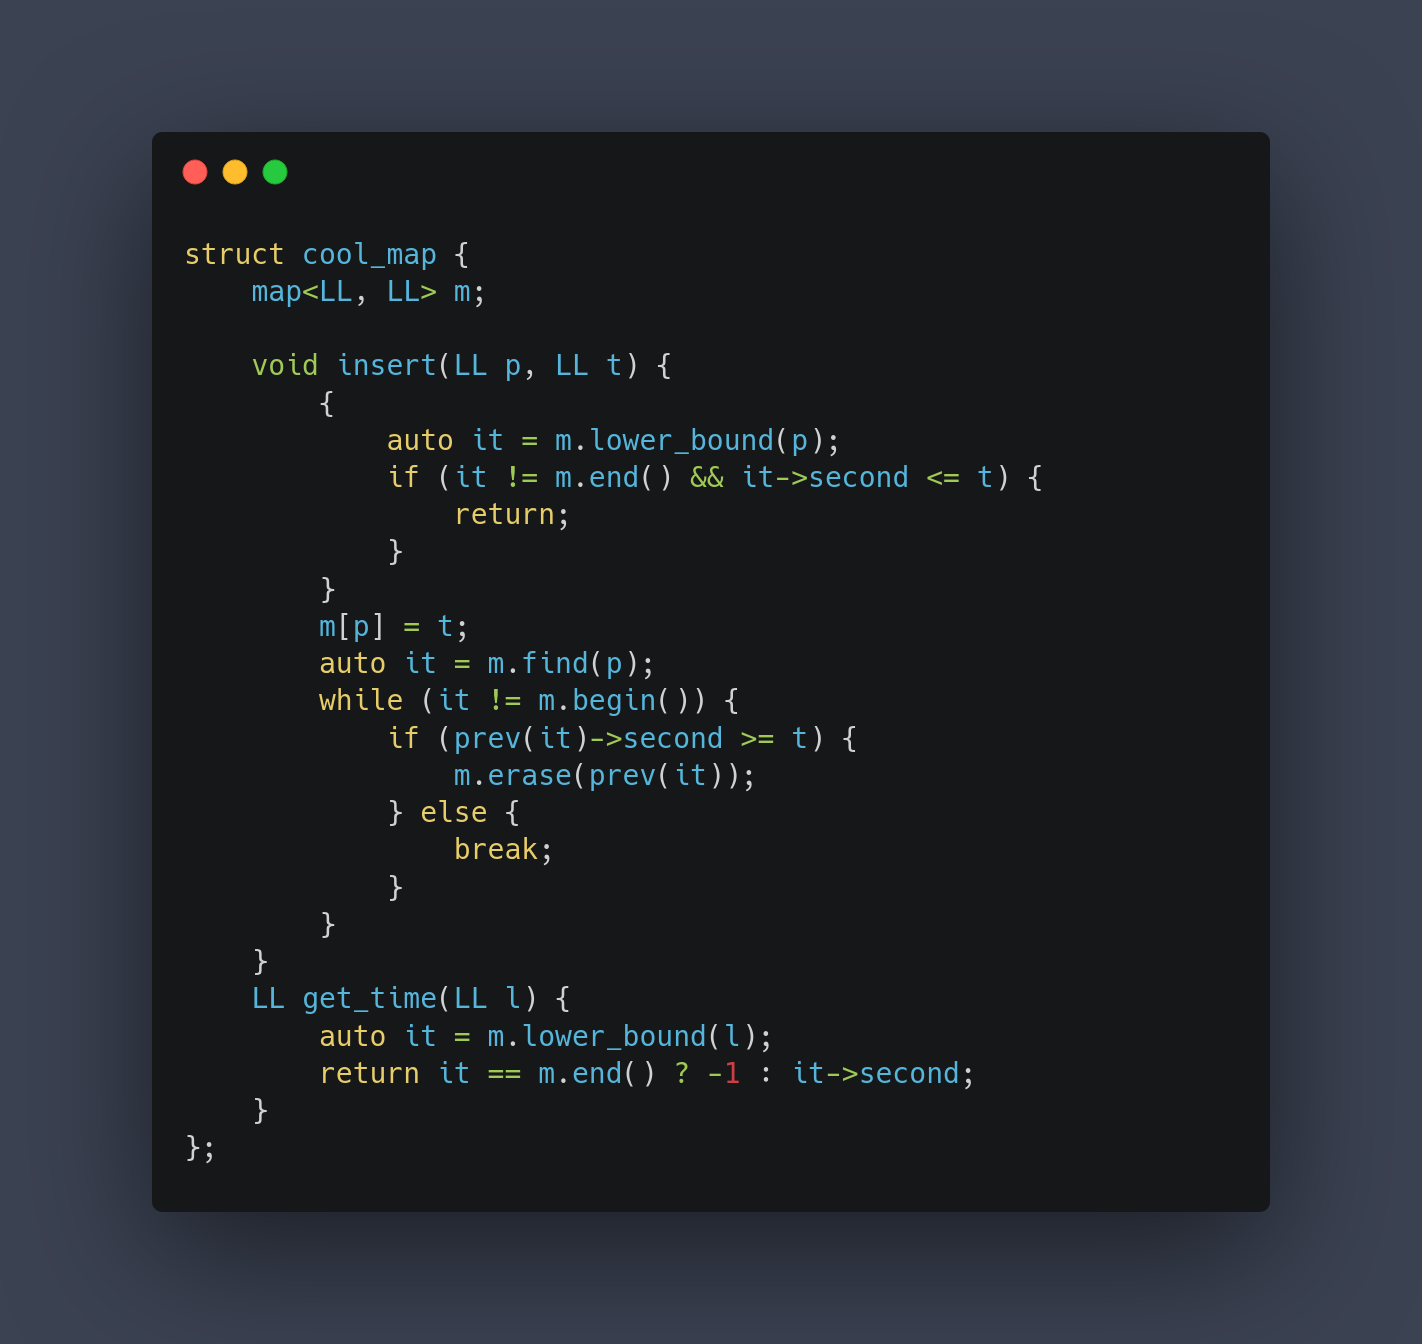
\includegraphics[scale=.2]{./img/cool_map_basic.png}}
\end{frame}

\begin{frame}{Problemi}{ois\_antennas}
    Abbiamo risolto il problema per $D = 0$, ma la potenza di ogni segnale diminuisce di $D$ ogni volta.

    \pause
    Manteniamo una variabile \texttt{d} che indica di quanto i segnali (le key) nella \texttt{map} sono maggiori rispetto ai segnali reali.
    \pause
    \begin{itemize}
        \item possiamo dimiuire tutti i segnali nella mappa semplicemente con \texttt{d += D}
        \item come possiamo inserire un segnale \texttt{p} al tempo \texttt{t}?
        \pause
        \begin{itemize}
            \pause
            \item tutti i segnali (key) sono maggiori di \texttt{d} rispetto ai segnali reali
            \pause
            \item non inseriamo la coppia \texttt{(p, t)}, ma \texttt{(p+d, t)}
        \end{itemize}
    \end{itemize}
\end{frame}

\begin{frame}{}
    \makebox[\textwidth]{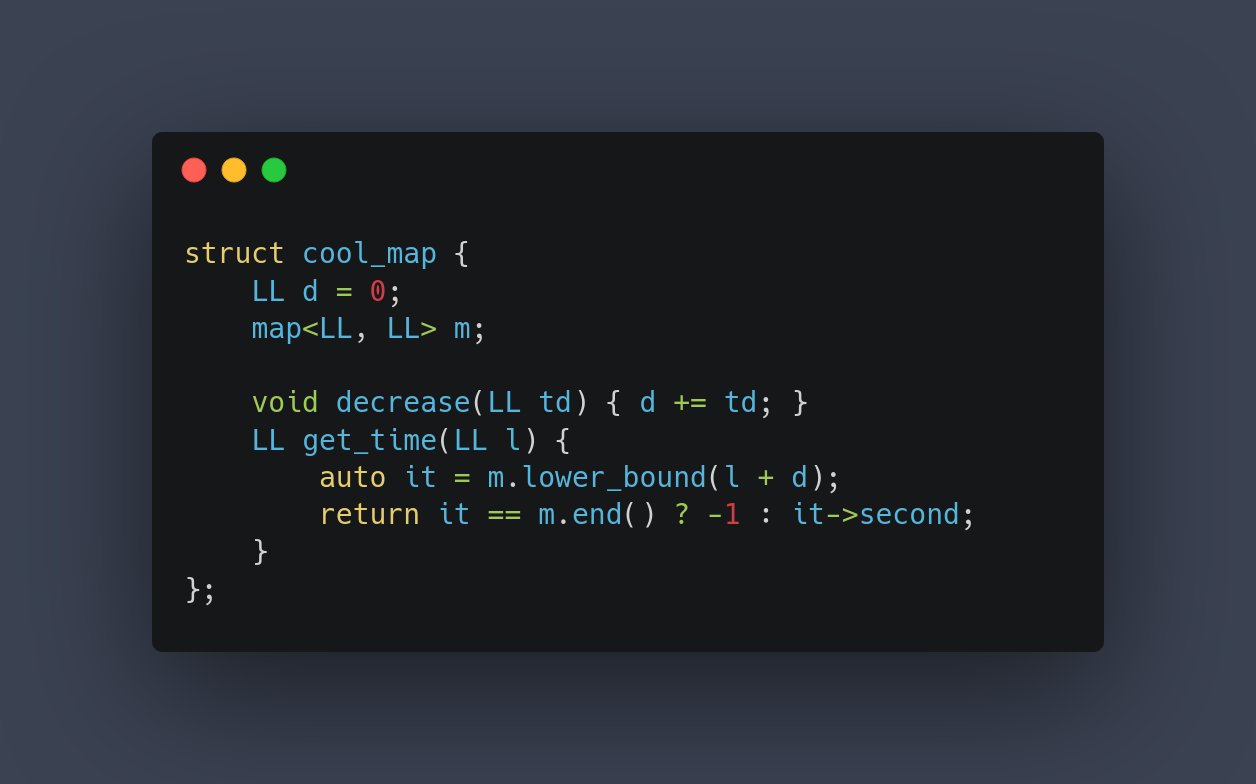
\includegraphics[scale=.25]{./img/cool_map_1.png}}
\end{frame}

\begin{frame}{}
    \makebox[\textwidth]{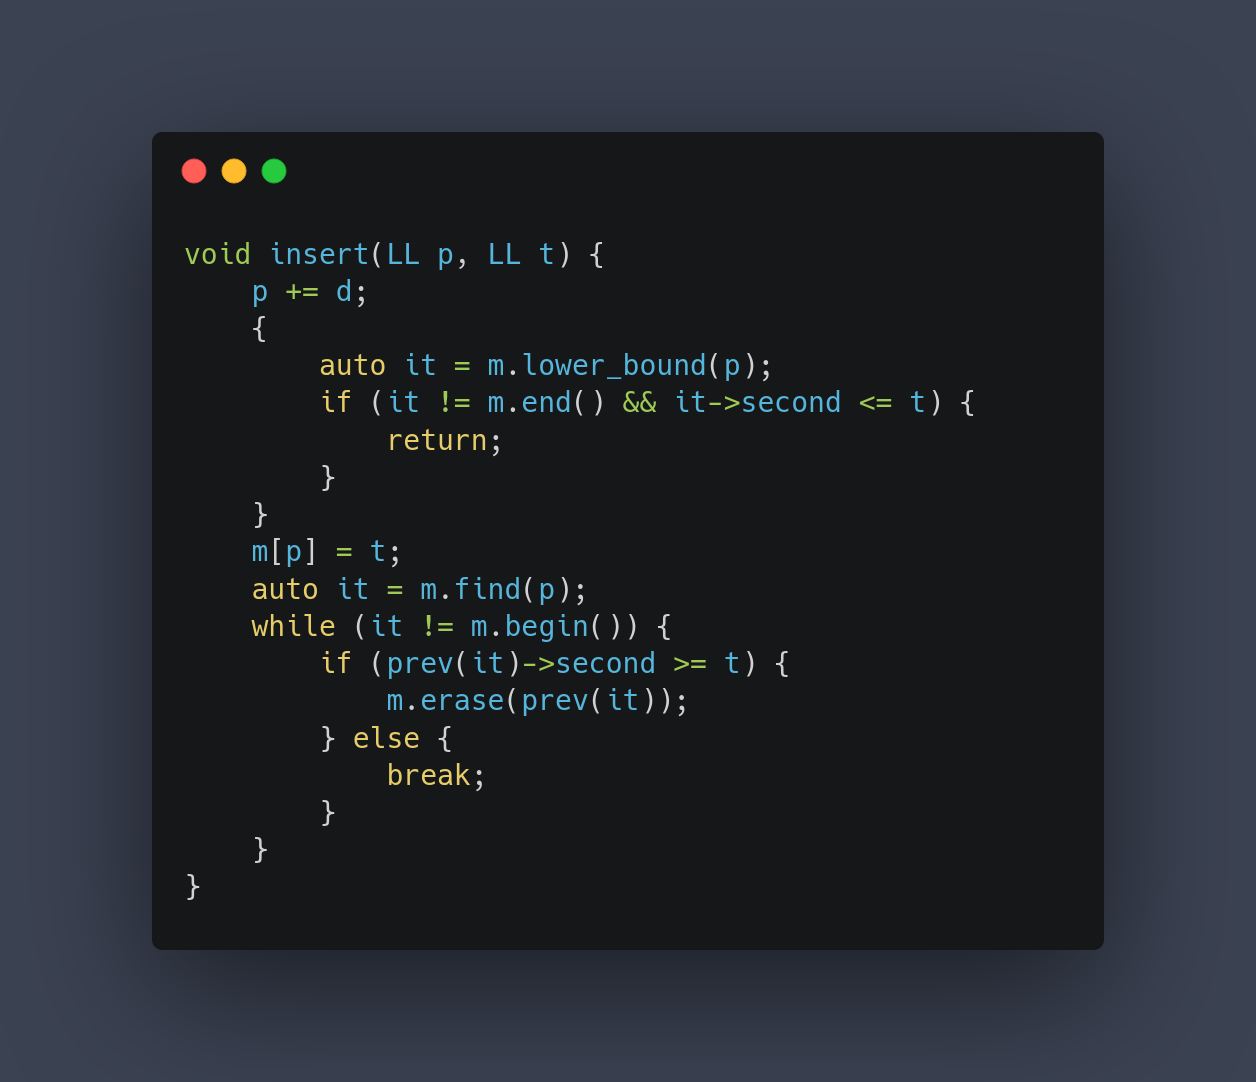
\includegraphics[scale=.25]{./img/cool_map_2.png}}
\end{frame}

\begin{frame}{Problemi}
    \underline{\url{https://cses.fi/problemset/task/2428}}
    \underline{\url{https://cses.fi/problemset/task/1630}}
    \underline{\url{https://cses.fi/problemset/task/1645}}
    \underline{\url{https://cses.fi/problemset/task/1661}}
    \underline{\url{https://cses.fi/problemset/task/2168}}
    \underline{\url{https://training.olinfo.it/\#/task/ois_antennas/statement}}
    \underline{\url{https://training.olinfo.it/\#/task/ois_videogame/statement}}
    \underline{\url{https://training.olinfo.it/\#/task/ois_intervals/statement}}
    \underline{\url{https://training.olinfo.it/\#/task/ois_wine/statement}}
    \underline{\url{https://training.olinfo.it/\#/task/preoii_pancake/statement}}
\end{frame}

\end{document}
